\chapter{Appendix: Theory and Methods}

\section{Procedure of BTCCD} \label{Appendix:ProcedureOfBTCCD}

\vfill
\begin{figure}[h]
	\centering
	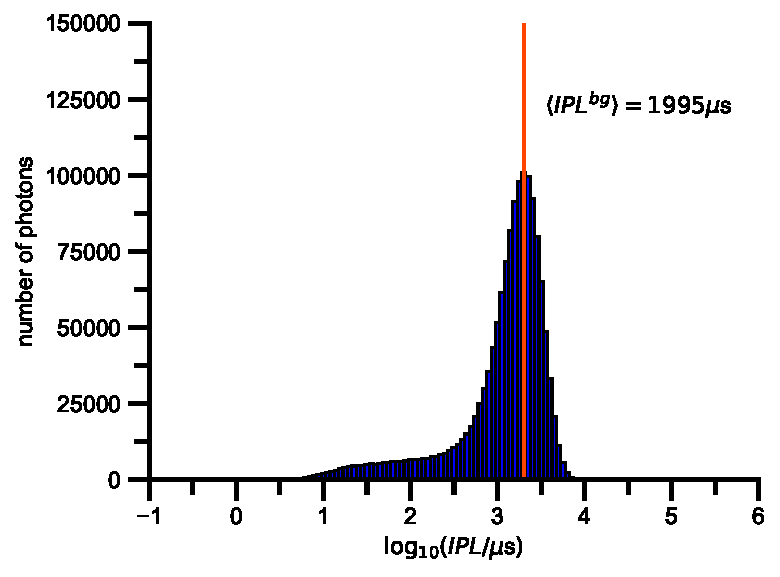
\includegraphics[width=4.8in]{dlDNA_IPD_Blue.pdf}
	\caption[Determination of background in \gls{IPL} time trace for blue channel]{Histogram of \gls{IPL} values for the blue channel. The right population reflects the background. In this case, it is characterized by $\left\langle IPL^{bg} \right\rangle = \SI{1995}{\micro\second}$ as indicated by the vertical orange line. The data is taken from a measurement of dual-labeled \gls{dsDNA}, see Section~\ref{Section:BTCCD_Measurement_Dependencies}.}
	\label{fig:IPLBackground_Blue}
\end{figure}  
\vfill
    
\vfill
\begin{figure}[h]
	\centering
	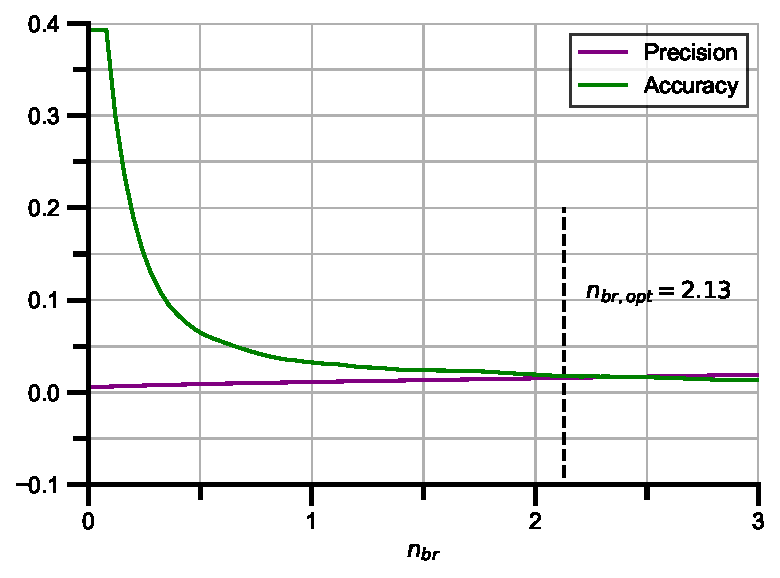
\includegraphics[width=4.8in]{OptimalBrightnessThresholdBlueChannel_dlDNA.pdf}
	\caption[Search for optimal brightness threshold $n_{br, opt}$ for blue channel]{Search for the optimal brightness threshold $n_{br, opt}$ for the blue channel. $n_{br, opt}$ is given by the intersection of precision and accuracy. The data is taken from a measurement of dual-labeled \gls{dsDNA}, see Section~\ref{Section:OptimalNumberOfBursts_Measurement}. In this case, $n_{br, opt}=\num{2.13}$ leads to a coincidence fraction of $f_{BR}(n_{br, opt}) = \SI{95.3 +- 1.7}{\percent}$.}
	\label{fig:OptimalBrightnessThresholdBlueChannel_dlDNA}
\end{figure}
\vfill
\clearpage

\section{Uncertainty on Dwell Time, Number of Molecules, and Molecular Brightness} \label{Appendix:UncertaintyDwellTime}

The average dwell time $\left\langle \tau_d \right\rangle$ is calculated from the single dwell times $\tau_{d,i}$ of $B$ selected bursts according to 
\begin{equation}
	\left\langle \tau_d \right\rangle (n_{br}) = \frac{1}{B(n_{br})} \sum_{i \in B(n_{br})} \tau_{d,i}. 
\end{equation}
Here, $i \in B(n_{br})$ denotes the sum over all selected bursts at a given brightness threshold. The uncertainty on a single dwell time $\tau_{d,i}$ is given by
\begin{equation}
	\sigma_{\tau_{d,i}} = \sqrt{\frac{1}{B(n_{br}) - 1} \sum_{j \in B(n_{br})} (\tau_{d,j} - \left\langle \tau_d \right\rangle (n_{br}))}.
\end{equation}
Then, the uncertainty on the average $\left\langle \tau_d \right\rangle$ decreases to 
\begin{equation}
	\sigma_{\left\langle \tau_d \right\rangle} (n_{br}) = \frac{\sigma_{\tau_{d,i}}}{\sqrt{B(n_{br})}}.
\end{equation}\\

The molecular brightness of a single burst is expressed by
\begin{equation}
	MB_i = \frac{N_{\gamma, i}}{\tau_{d, i}},
\end{equation}
where $N_{\gamma, i}$ denotes the number of photons in the i-th burst. Since $N_{\gamma, i}$ is Poisson distributed, its uncertainty is given by $\sigma_{N_{\gamma, i}} = \sqrt{N_{\gamma, i}}$. The average molecular brightness is derived by
\begin{equation}
	\left\langle MB \right\rangle (n_{br}) = \frac{1}{B(n_{br})} \sum_{i \in B(n_{br})} MB_i.
\end{equation}
Thus, the uncertainty of $N_{\gamma, i}$ and $\tau_{d, i}$ propagate on $\left\langle MB \right\rangle$ by
\begin{align}
	\sigma_{\left\langle MB \right\rangle} (n_{br}) &= \sqrt{\sum_{i \in B(n_{br})} \left \{ \left(\frac{\sigma_{N_{\gamma, i}}}{N_{\gamma,i}}\right)^2 + \left(\frac{\sigma_{\tau_{d, i}}}{\tau_{d, i}}\right)^2 + \left(\frac{\sigma_{B}(n_{br})}{B(n_{br})}\right)^2 \right \} }\\
	& = \sqrt{\sum_{i \in B(n_{br})} \left\{ \frac{1}{N_{\gamma,i}} + \left(\frac{\sigma_{\tau_{d, i}}}{\tau_{d, i}}\right)^2 + \frac{1}{B(n_{br})}\right\}}.
\end{align}\\

Finally, since $\left\langle N \right\rangle$ is calculated by \eqref{Equation:AverageNumberOfMolecules}, its uncertainty is given by
\begin{align}
	\sigma_{\left\langle N \right\rangle} (n_{br}) &= \frac{1}{1 - \frac{B(n_{br}) \cdot \left\langle \tau_d \right\rangle (n_{br})}{T}} \sqrt{\left(\frac{\left\langle \tau_d \right\rangle (n_{br})}{T} \sigma_B (n_{br})\right)^2 + \left(\frac{B(n_{BR}) (n_{br})}{T} \sigma_{\left\langle \tau_d \right\rangle} (n_{br})\right)^2 } \\
	&= \frac{1}{1 - \frac{B(n_{br}) \cdot \left\langle \tau_d \right\rangle (n_{br})}{T}} \sqrt{\left(\frac{\left\langle \tau_d \right\rangle (n_{br})}{T} \sqrt{B (n_{br})}\right)^2 + \left(\frac{B(n_{BR}) (n_{br})}{T} \sigma_{\left\langle \tau_d \right\rangle} (n_{br})\right)^2 }
\end{align}

\clearpage

\section{Uncertainty on Corrected Coincidence Fraction} \label{Appendix:UncertaintyOnChanceCoincidenceCorrection}

Formally, the uncertainty on $f_{RB}^{cor}$ can be expressed by
\begin{equation}
\sigma_{f_{RB}^{cor}}(n_{br}) = f_{RB}^{cor}(n_{br}) \sqrt{\frac{\left(\sigma_{f_{RB}}(n_{br})\right)^2 + \left(\sigma_{f_{RB, 0}^{chance}}(n_{br})\right)^2}{\left(f_{RB}(n_{br}) - f_{RB, 0}^{chance}(n_{br})\right)^2} + \frac{\left(\sigma_{f_{RB, 0}^{chance}}(n_{br})\right)^2}{\left(1 - f_{RB, 0}^{chance}(n_{br})\right)^2}}.
\end{equation}
According to Equation~\eqref{Equation:UncertaintyCoincidenceFractionRed}, the uncertainty on the uncorrected coincidence fraction $f_{RB}$ is given by
\begin{equation*}
\sigma_{f_{RB}}(n_{br}) = f_{RB}(n_{br}) \cdot \sqrt{\frac{1}{B_{RB}(n_{br})} + \frac{1}{B_{R}(n_{br})}},
\end{equation*}
where $B_{R}$ is the total number of selected red bursts and $B_{RB}$ is the number of coincident bursts. The uncertainty on $f_{RB}^{chance}$ still needs to be determined. It can be expressed by
\begin{equation}
\begin{aligned}
\sigma_{f_{RB, 0}^{chance}}(n_{br}) = & \exp\left\{-\left\langle N_B \right\rangle (0) \cdot \left(\frac{\left\langle \tau_d^R \right\rangle (n_{br})}{\left\langle \tau_d^B \right\rangle (0)} + 1\right)\right\} \times \\  
& \left\{ \left(\frac{\left\langle \tau_d^R \right\rangle (n_{br})}{\left\langle \tau_d^B \right\rangle (0)} + 1\right)^2 \cdot \left(\sigma_{\left\langle N_B \right\rangle}(0)\right)^2 + \left(\frac{\left\langle N_B \right\rangle(0)}{\left\langle \tau_d^B \right\rangle (0)} \sigma_{\left\langle \tau_d^R \right\rangle}(n_{br})\right)^2 + \right.\\
& \left. \left( \frac{\left\langle N_B \right\rangle(0)\left\langle \tau_d^R \right\rangle (n_{br})}{\left(\left\langle \tau_d^B \right\rangle (0)\right)^2} \sigma_{\left\langle \tau_d^B \right\rangle}(0)\right)^2\right\}^{1/2}.
\end{aligned}
\end{equation}

The result can also be used to determine the uncertainty $\sigma_{f_{BR}^{cor}}$ on $f_{BR}^{cor}$ by substituting ${RB \rightarrow BR}$.

\chapter{Appendix: Dependencies on Brightness Threshold} 

\section{Dwell Time} 

\vfill
\begin{figure}[h]
	\centering
	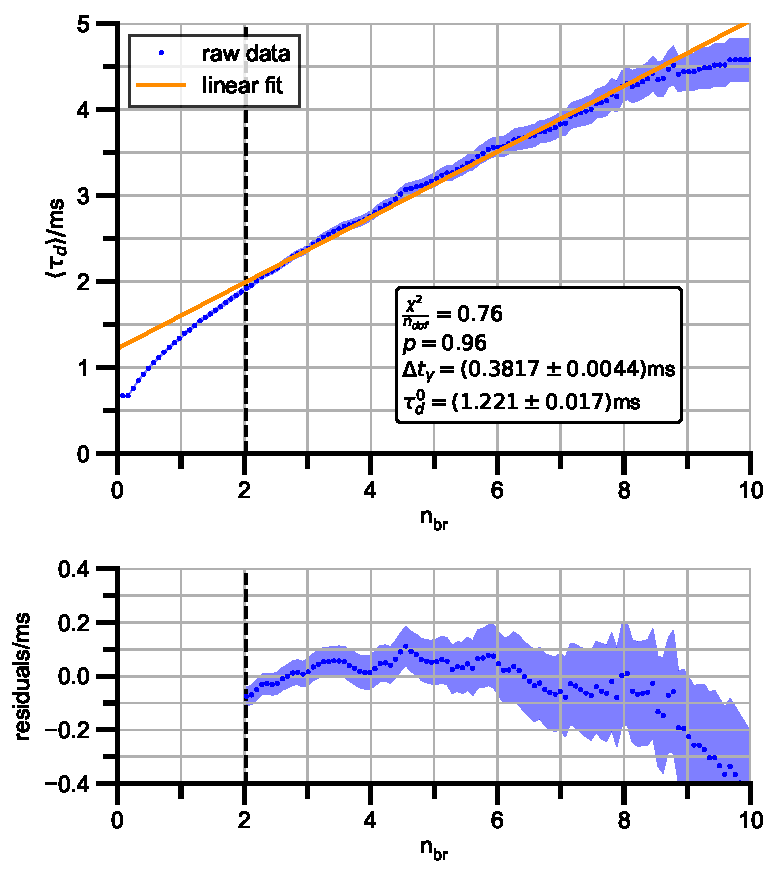
\includegraphics[width=4.8in]{CheckDependencies_DwellTimeBlue_Theory.pdf}
	\caption[Linear fit of dwell time for blue channel]{Linear fit according to $\left\langle \tau_d \right\rangle (n_{br}) =  \tau_d^0 + \Delta t_{\gamma} \cdot n_{br}$ for the blue channel. Information on the measurement can be found in Section~\ref{Section:BTCCD_Measurement_Dependencies}. The vertical dashed line indicates the range of $n_{br}$ that was used for fitting. For smaller $n_{br}$, the dependency is not linear. For higher $n_{br}$, the residual plot reveals a slight deviation of the fitted model from the raw data.}
	\label{fig:CheckDependencies_DwellTimeBlue_Theory}
\end{figure}
\vfill

\vfill
\begin{figure}[h]
	\centering
	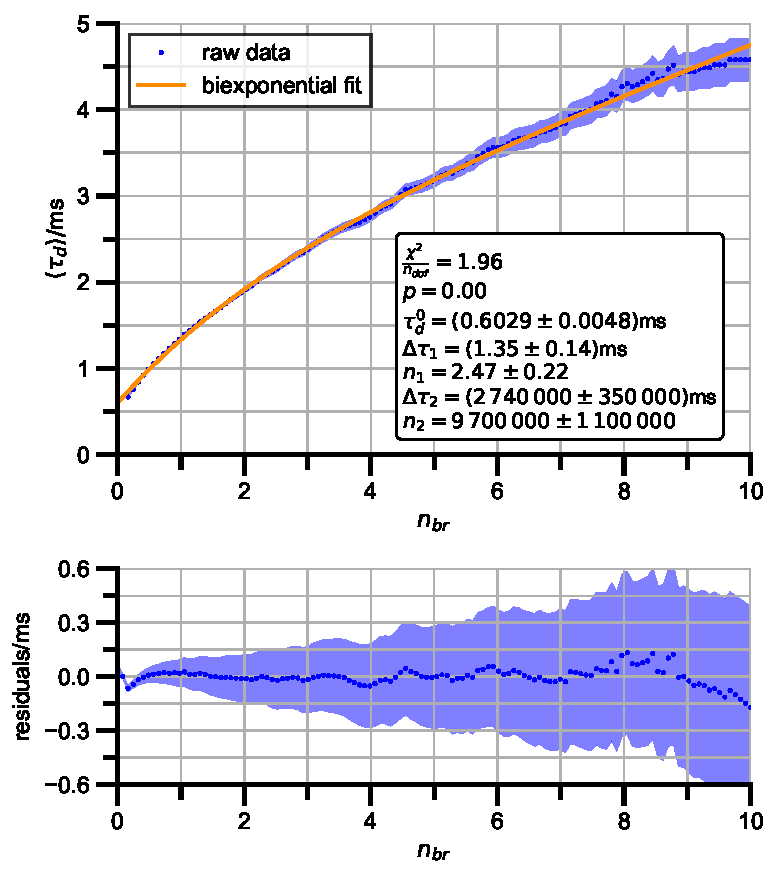
\includegraphics[width=4.8in]{CheckDependencies_DwellTimeBlue_Experiment.pdf}
	\caption[Biexponential fit of dwell time for blue channel]{Biexponential fit according to $\left\langle \tau_d \right\rangle (n_{br}) = \tau_d^0 + \Delta \tau_1 (1 - e^{-n_{br}/ n_1}) + \Delta \tau_2 (1 - e^{-n_{br}/ n_2})$ for the blue channel. Information on the measurement can be found in Section~\ref{Section:BTCCD_Measurement_Dependencies}. The biexponential function takes two different saturation processes into account. For the blue channel, $\tau_2$ and $n_2$ are notably large. Thus, the second exponential term effectively describes a linear function. The slope is in agreement with the result from the linear fit, see Section~\ref{Section:PropertiesDwellTime}.}
	\label{fig:CheckDependencies_DwellTimeBlue_Experiment}
\end{figure}
\vfill

\clearpage

\section{Number of Molecules} 

\vfill
\begin{figure}[h]
	\centering
	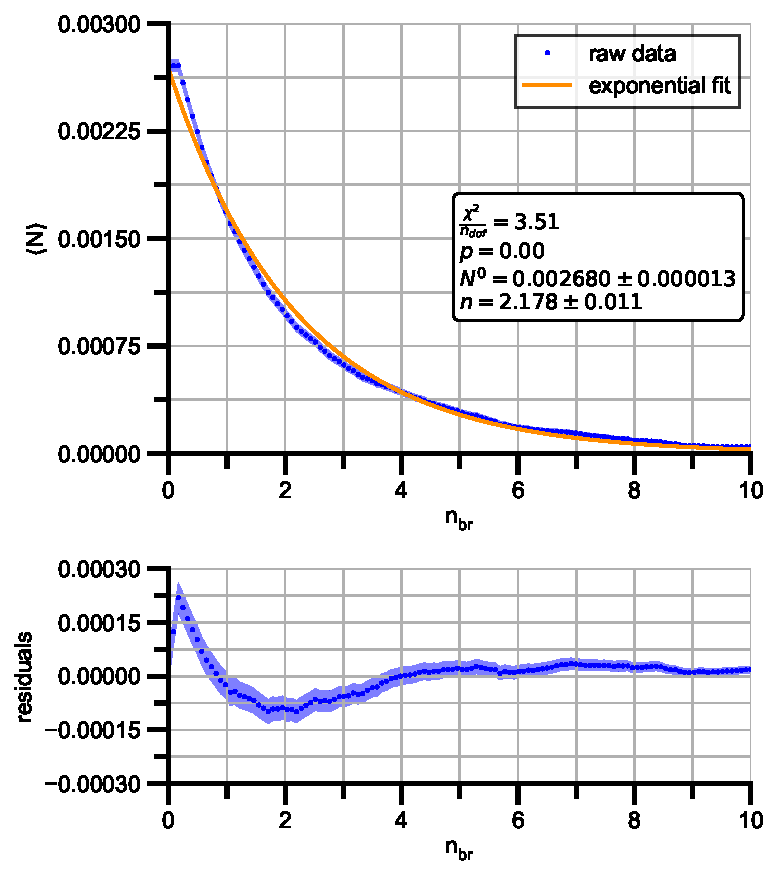
\includegraphics[width=4.8in]{CheckDependencies_NumberMoleculesBlue_Theory.pdf}
	\caption[Exponential fit of molecule number for blue channel]{Exponential fit according to $\left\langle N \right\rangle (n_{br}) = N^0e^{-n_{br}/ n}$ for the blue channel. Information on the measurement can be found in Section~\ref{Section:BTCCD_Measurement_Dependencies}. The fit reflects the general decreasing trend of $\left\langle N \right\rangle$, but deviates clearly from the specific behavior.}
	\label{fig:CheckDependencies_NumberMoleculesBlue_Theory}
\end{figure}
\vfill

\vfill
\begin{figure}[h]
	\centering
	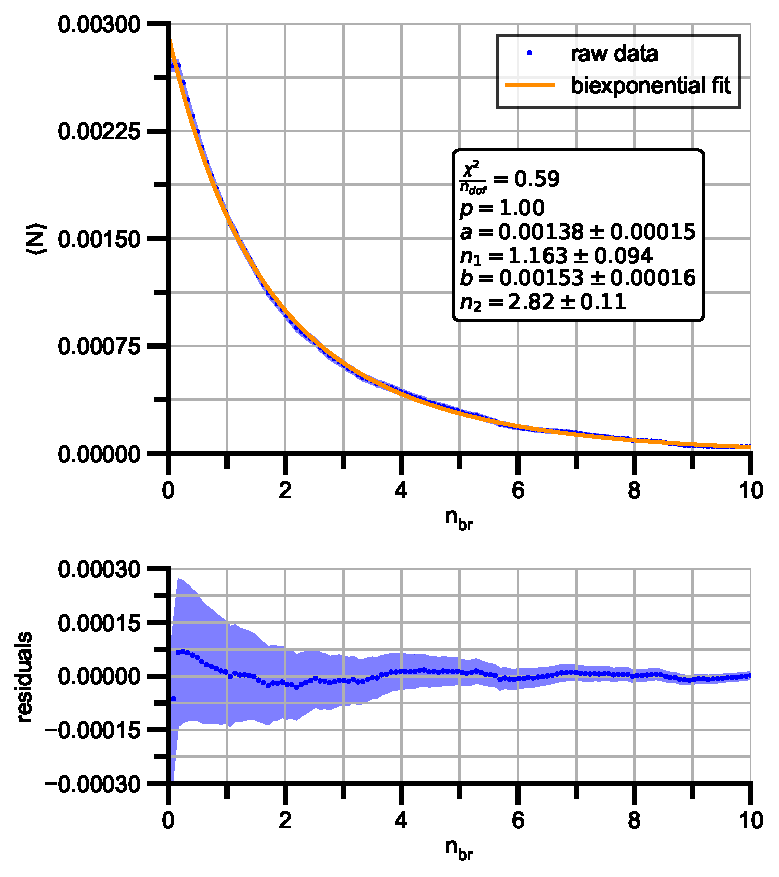
\includegraphics[width=4.8in]{CheckDependencies_NumberMoleculesBlue_Experiment.pdf}
	\caption[Biexponential fit of molecule number for blue channel]{Biexponential fit according to $\left\langle N \right\rangle (n_{br}) = ae^{-n_{br}/ n_1} + be^{-n_{br}/ n_2}$ for the blue channel. Information on the measurement can be found in Section~\ref{Section:BTCCD_Measurement_Dependencies}. The two decay processes of the biexponential function modulate the measurement more accurately than the monoexponential model.}
	\label{fig:CheckDependencies_NumberMoleculesBlue_Experiment}
\end{figure}
\vfill

\clearpage

\section{Molecular Brightness} 

\vfill
\begin{figure}[h!]
	\centering
	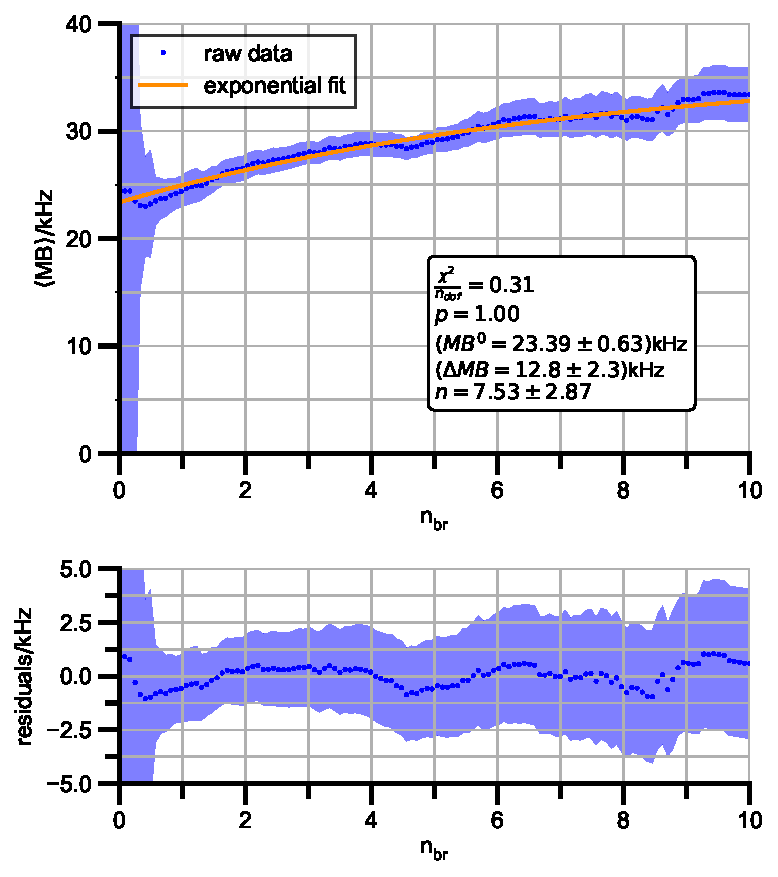
\includegraphics[width=4.8in]{CheckDependencies_MolecularBrightnessBlue_Theory.pdf}
	\caption[Exponential fit of molecular brightness for blue channel]{Exponential fit according to $\left\langle MB \right\rangle (n_{br}) = MB^0 + \Delta MB(1 - e^{-n_{br}/ n})$ for the blue channel. Information on the measurement can be found in Section~\ref{Section:BTCCD_Measurement_Dependencies}. The model describes the raw data accurately. The comparably large uncertainty on $\left\langle MB \right\rangle$ explains the low value for $\chi^2/ n_{dof}$ for the fits.}
	\label{fig:CheckDependencies_MolecularBrightnessBlue_Theory}
\end{figure}
\vfill

\vfill
\begin{figure}[h]
	\centering
	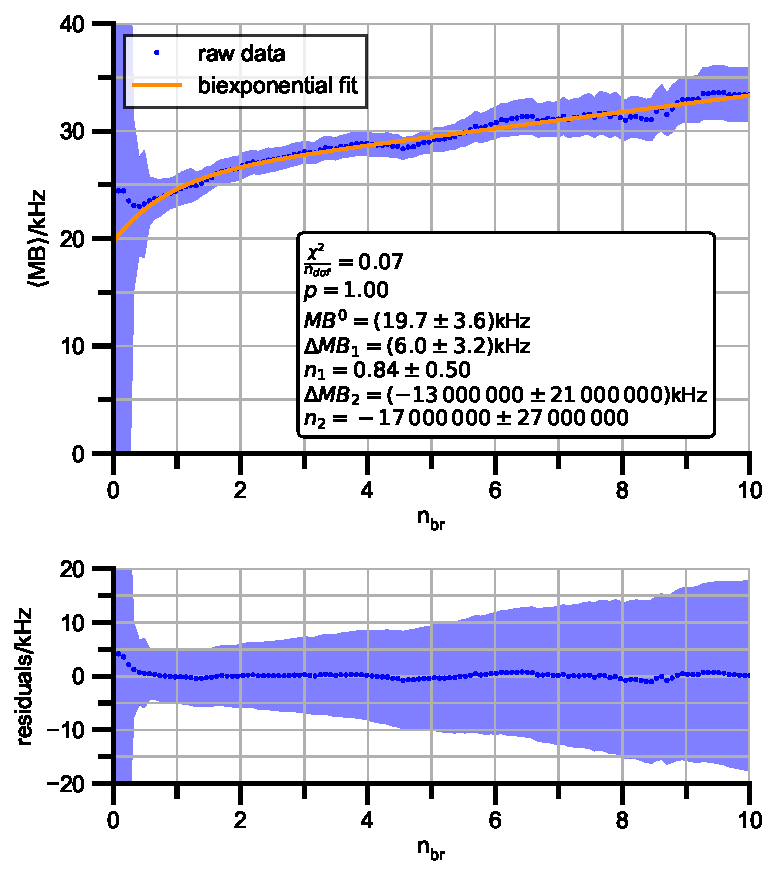
\includegraphics[width=4.8in]{CheckDependencies_MolecularBrightnessBlue_Experiment.pdf}
	\caption[Biexponential fit of molecular brightness for blue channel]{Fit according to $\left\langle MB \right\rangle (n_{br}) = MB^0 + \Delta MB_1(1 - e^{-n_{br}/ n_1}) + \Delta MB_2(1 - e^{-n_{br}/ n_2})$ for the blue channel. Information on the measurement can be found in Section~\ref{Section:BTCCD_Measurement_Dependencies}. The parameters of the second exponential term are in agreement with zero. Therefore, for the blue channel, the molecular brightness is effectively described by a monoexponential saturation.}
	\label{fig:CheckDependencies_MolecularBrightnessBlue_Experiment}
\end{figure}
\vfill

\chapter{Appendix: Optimal Number of Bursts}

\vfill
\begin{figure}[h]
	\centering
	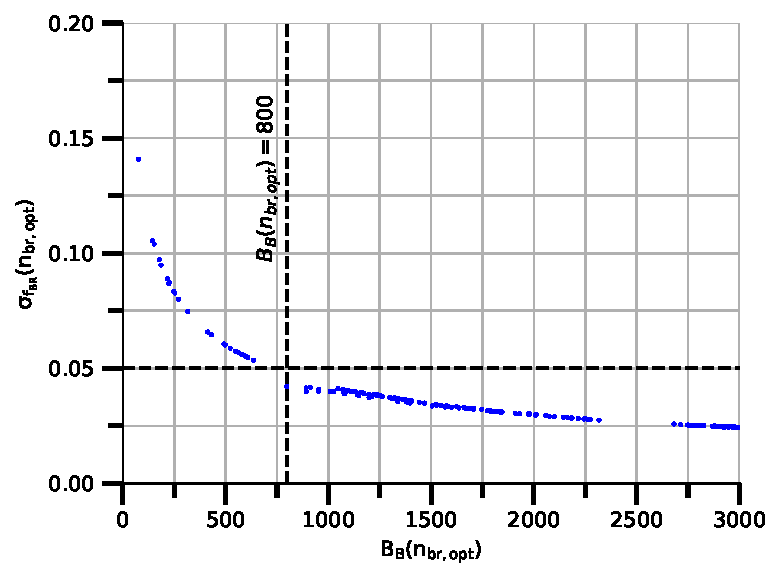
\includegraphics[width=4.8in]{OptimalNumberOfSelectedBurstsBlue.pdf}
	\caption[Optimal number of selected bursts for blue channel]{Uncertainty on the coincidence fraction $f_{BR}$ at the optimal brightness threshold $n_{br,opt}$ as a function of the selected number of bursts $B_B(n_{br,opt})$ for the blue channel. Information on the measurement can be found in Section~\ref{Section:OptimalNumberOfBursts_Measurement}. The optimal number of selected bursts, for which the uncertainty falls below \SI{5}{\percent}, is approximately $B_B(n_{br,opt}) = 800$.}
	\label{fig:SelectedNumberOfBurstsBlue}
\end{figure} 
\vfill

\vfill
\begin{figure}[h]
	\centering
	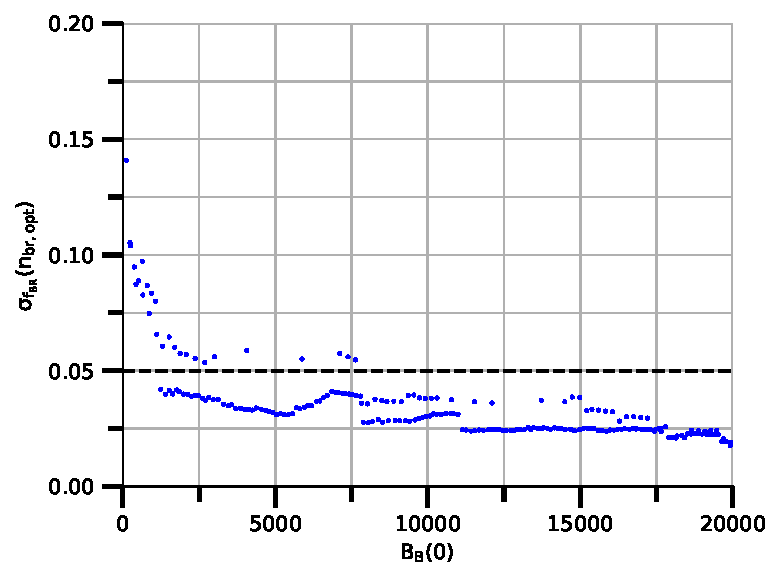
\includegraphics[width=4.8in]{OptimalNumberOfTotalBurstsBlue.pdf}
	\caption[Optimal number of initial bursts for blue channel]{Uncertainty on the coincidence fraction $f_{BR}$ at the optimal brightness threshold $n_{br,opt}$ as a function of the initial number of bursts $B_B(0)$ for the blue channel. Information on the measurement can be found in Section~\ref{Section:OptimalNumberOfBursts_Measurement}. The graph does not reveal a completely deterministic behavior. However, for a number of about \num{7500} initial bursts, the uncertainty is typically lower than \SI{5}{\percent}.}
	\label{fig:TotalNumberOfBurstsBlue}
\end{figure} 
\vfill

\chapter{Appendix: Chance Coincidence Limitation}

\section{Application Limits of Chance Coincidence Correction}

\vfill
\begin{figure}[h]
	\centering
	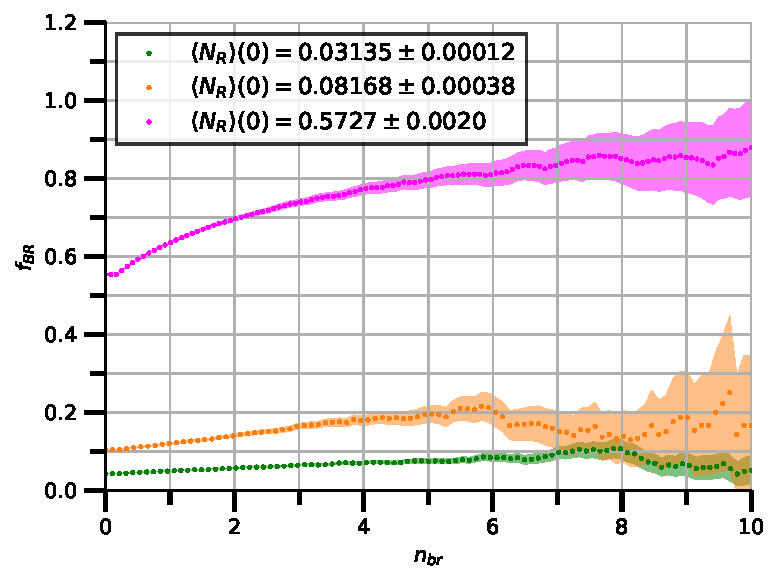
\includegraphics[width=4.8in]{CoincidenceFraction_DNA_Blue.pdf}
	\caption[Coincidence fraction of blue channel for mixture of red-labeled \gls{dsDNA} and free blue dye]{Coincidence fraction of blue channel $f_{BR}$ for the mixture of red-labeled \gls{dsDNA} and free blue dye for a small, intermediate, and high molecule number. Information on the measurement can be found in Section~\ref{Section:Measurement_Ribosomes_DNA}. The observed coincidence fraction is primarily caused by chance coincidences and increases with $\left\langle N_R \right\rangle (0)$ and $n_{br}$.}
	\label{fig:CoincidenceFraction_DNA_Blue}
\end{figure}
\vfill

\vfill
\begin{figure}[h]
	\centering
	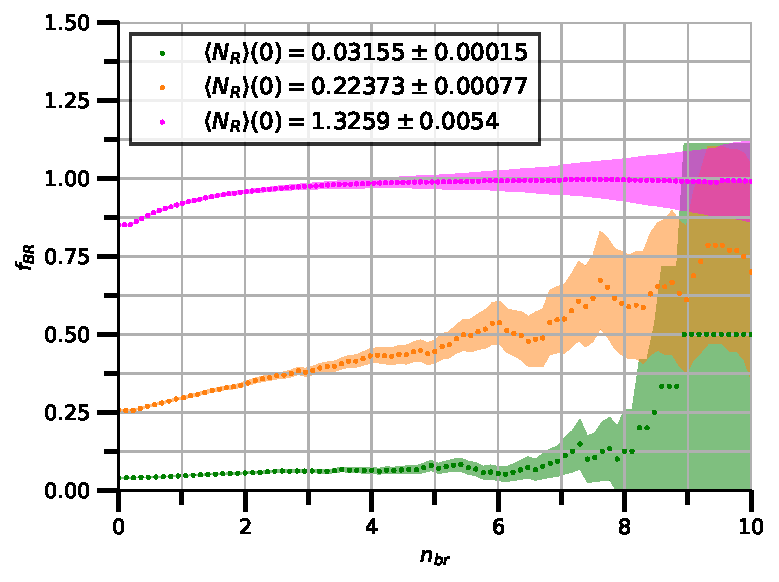
\includegraphics[width=4.8in]{CoincidenceFraction_Ribosomes_Blue.pdf}
	\caption[Coincidence fraction of blue channel for mixture of red-labeled ribosomes and free blue dye]{Coincidence fraction of blue channel $f_{BR}$ for the mixture of red-labeled ribosomes and free blue dye for a small, intermediate, and high molecule number. Information on the measurement can be found in Section~\ref{Section:Measurement_Ribosomes_DNA}. The observed coincidence fraction is primarily caused by chance coincidences and increases with $\left\langle N_R \right\rangle (0)$ and $n_{br}$.}
	\label{fig:CoincidenceFraction_Ribosomes_Blue}
\end{figure}
\vfill

\vfill
\begin{figure}[h]
	\centering
	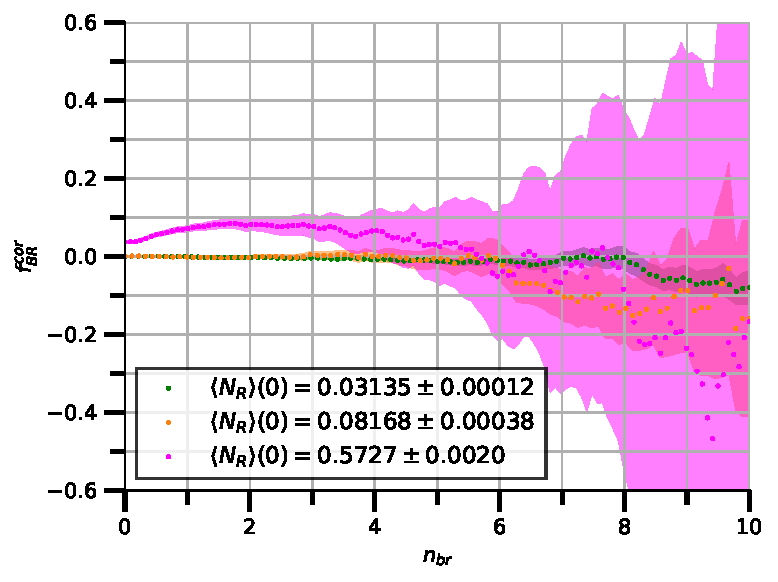
\includegraphics[width=4.8in]{CorrectedCoincidenceFraction_DNA_Blue.pdf}
	\caption[Corrected coincidence fraction of blue channel for mixture of red-labeled \gls{dsDNA} and free blue dye]{Corrected coincidence fraction of blue channel $f_{BR}^{cor}$ for the mixture of red-labeled \gls{dsDNA} and free blue dye for a low, intermediate, and high molecule number. Information on the measurement can be found in Section~\ref{Section:Measurement_Ribosomes_DNA}. For the highest molecule number, the corrected coincidence fraction deviates slightly from the expected value of \SI{0}{\percent}. However, more pronounced is the uncertainty that - compared to the red channel - becomes extremely large for high brightness thresholds. It is caused by a smaller amount of bursts in the blue channel.}
	\label{fig:CorrectedCoincidenceFraction_DNA_Blue}
\end{figure}
\vfill

\vfill
\begin{figure}[h]
	\centering
	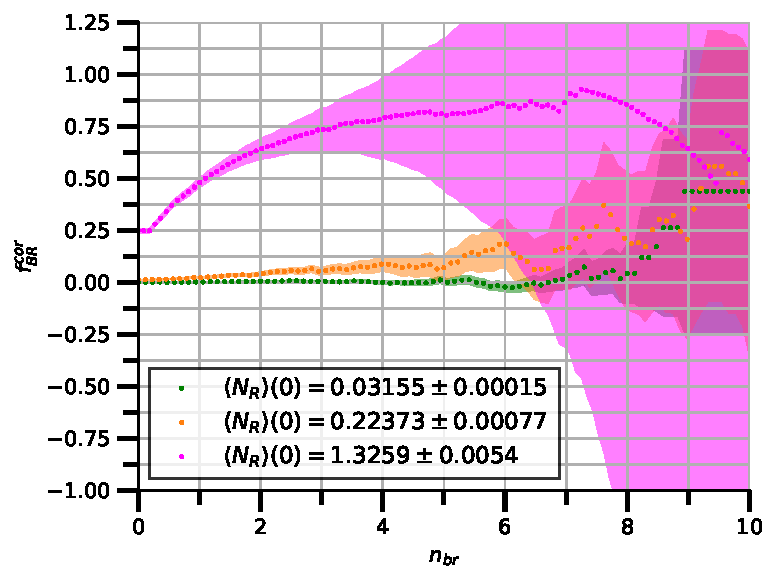
\includegraphics[width=4.8in]{CorrectedCoincidenceFraction_Ribosomes_Blue.pdf}
	\caption[Corrected coincidence fraction of blue channel for mixture of red-labeled ribosomes and free blue dye]{Corrected coincidence fraction of blue channel $f_{BR}^{cor}$ for the mixture of red-labeled ribosomes and free blue dye for a low, intermediate, and high molecule number. Information on the measurement can be found in Section~\ref{Section:Measurement_Ribosomes_DNA}. Only for the highest molecule number, the corrected coincidence fraction deviates significantly from the expected value of \SI{0}{\percent}. However, more pronounced is the uncertainty that - compared to the red channel - becomes extremely large for high brightness thresholds. It is caused by a smaller amount of bursts in the blue channel.}
	\label{fig:CorrectedCoincidenceFraction_Ribosomes_Blue}
\end{figure}
\vfill

\vfill
\begin{figure}[h]
	\centering
	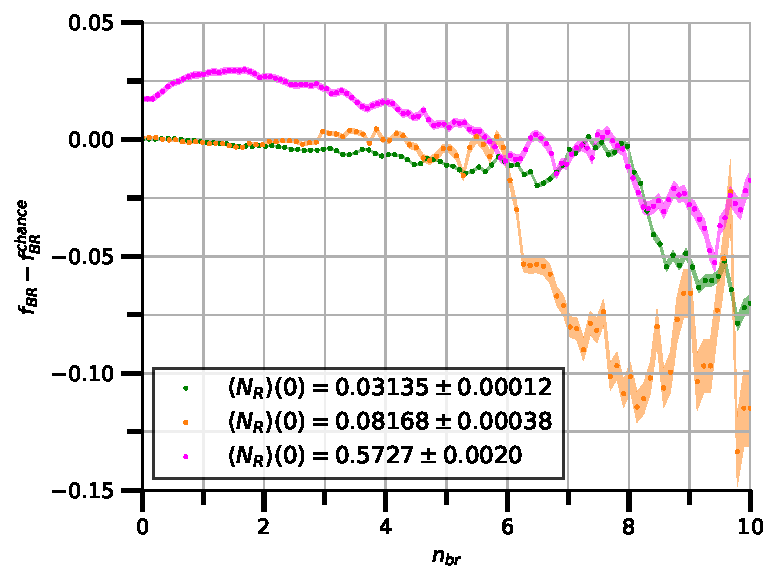
\includegraphics[width=4.8in]{ChanceCoincidenceFraction_DNA_Blue.pdf}
	\caption[First term of corrected coincidence fraction of blue channel for mixture of red-labeled \gls{dsDNA} and free blue dye]{First term of corrected coincidence fraction of blue channel $f_{BR} - f_{BR,0}^{chance}$ for the mixture of red-labeled \gls{dsDNA} and free blue dye for a small, intermediate, and high molecule number. Information on the measurement can be found in Section~\ref{Section:Measurement_Ribosomes_DNA}. For large $n_{br}$, the first term deviates clearly from the expected value of \SI{0}{\percent}. There, the number of bursts is low and explains the deviation.}
	\label{fig:ChanceCoincidenceFraction_DNA_Blue}
\end{figure}
\vfill

\vfill
\begin{figure}[h]
	\centering
	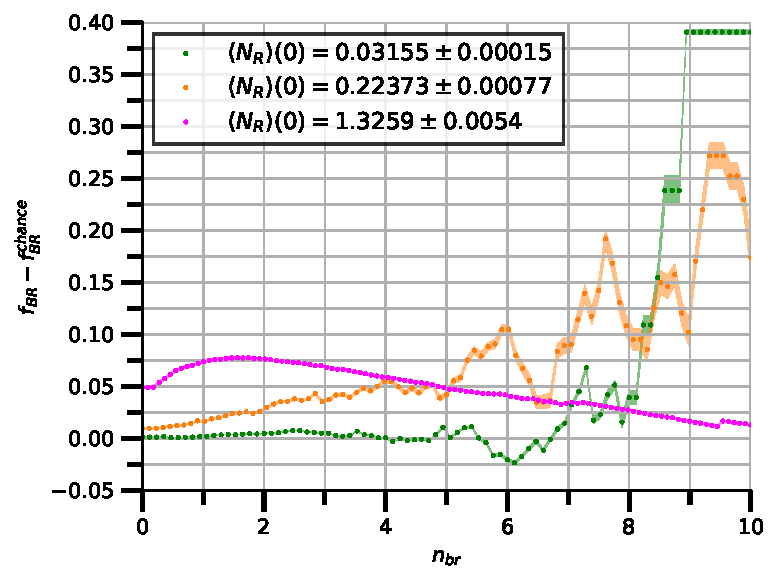
\includegraphics[width=4.8in]{ChanceCoincidenceFraction_Ribosomes_Blue.pdf}
	\caption[First term of corrected coincidence fraction of blue channel for mixture of red-labeled ribosomes and free blue dye]{First term of corrected coincidence fraction of blue channel $f_{BR} - f_{BR,0}^{chance}$ for the mixture of red-labeled ribosomes and free blue dye for a small, intermediate, and high molecule number. Information on the measurement can be found in Section~\ref{Section:Measurement_Ribosomes_DNA}. For large $n_{br}$, the first term deviates clearly from the expected value of \SI{0}{\percent}. There, the number of bursts is low and explains the deviation.}
	\label{fig:ChanceCoincidenceFraction_Ribosomes_Blue}
\end{figure}
\vfill

\vfill
\begin{figure}[h]
	\centering
	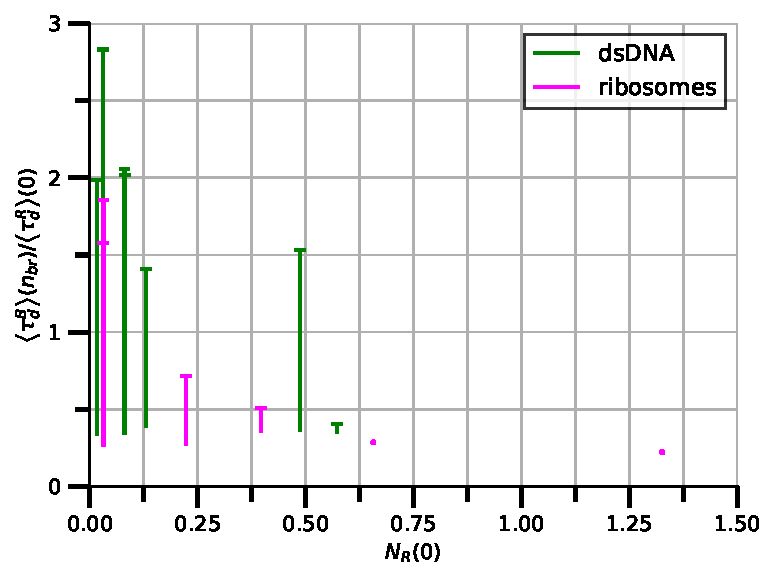
\includegraphics[width=4.8in]{PossibleRanges_Blue.pdf}
	\caption[Application range of chance coincidence correction for blue channel for measurements with \gls{dsDNA} and ribosomes]{Application range in terms of dwell time ratio as a function of the molecule number for the blue channel. Information on the measurements with \gls{dsDNA} and ribosomes can be found in Section~\ref{Section:Measurement_Ribosomes_DNA}. Every vertical line represents one measurement. A short horizontal line at the highest dwell time ratio indicates that the deviation of the corrected coincidence fraction or its statistical uncertainty becomes more than \SI{5}{\percent} for higher dwell time ratios. A simple dot denotes that the chance coincidence correction is unsuitable for the whole measurement.}
	\label{fig:PossibleRanges_Blue}
\end{figure}
\vfill

\vfill
\begin{figure}[h]
	\centering
	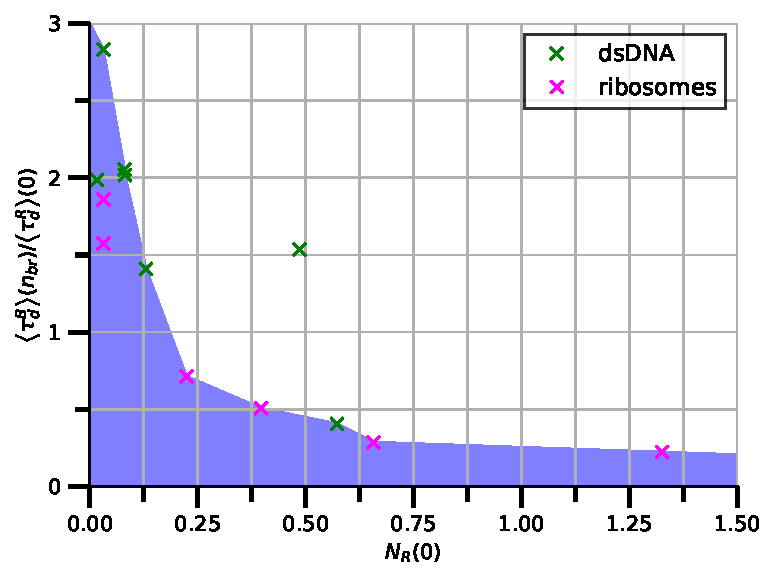
\includegraphics[width=4.8in]{ReferenceGraph_Blue.pdf}
	\caption[Interpolated application range of chance coincidence correction for blue channel for measurements with \gls{dsDNA} and ribosomes]{Interpolated application range in terms of dwell time ratio as a function of the molecule number for the blue channel. Information on the measurements with \gls{dsDNA} and ribosomes can be found in Section~\ref{Section:Measurement_Ribosomes_DNA}. The interpolation serves only for illustration and is not derived from theoretical knowledge. It allows to determine the application range for an arbitrary molecule number.}
	\label{fig:ReferenceGraph_Blue}
\end{figure}
\vfill
\clearpage

\section{Validation of Application Limits}

\vfill
\begin{table}[h]
	\centering
	\begin{tabular}{c|c|c|c|c} 
		$n_{br,opt}$ & $\left\langle N_R \right\rangle (0)$ [$10^{-3}$] & $\left\langle \tau_d^B \right\rangle(n_{br,opt})/ \left\langle \tau_d^R  \right\rangle(0)$ & $f_{BR}(n_{br,opt})$ [\si{\percent}] & $f_{BR}^{cor}(n_{br,opt})$ [\si{\percent}] \\
		\hline
		\num{1.30} & \num{18.47 +- 0.11} & \num{1.398 +- 0.011} & \num{84.2 +- 2.1} & \num{83.5+- 2.2} \\
		\num{3.52} & \num{26.54 +- 0.13} & \num{1.807 +- 0.011} & \num{85.6 +- 2.9} & \num{84.5+- 3.2} \\
		\num{1.95} & \num{94.56 +- 0.56} & \num{1.4415 +- 0.0091} & \num{90.6 +- 2.2} & \num{88.2+- 2.7} \\
		\num{2.00} & \num{126.83 +- 0.56} & \num{1.4124 +- 0.0083} & \num{91.5 +- 2.0} & \num{88.4+- 2.7} \\
		\num{0.87} & \num{621.7 +- 2.0} & \num{1.3982 +- 0.0043} & \num{97.44 +- 0.64} & \num{88.6+- 2.9} \\ 
		\num{3.72} & \num{777.8 +- 2.8} & \num{2.6371 +- 0.0057} & \num{99.6 +- 1.7} & \num{93+- 28} 
	\end{tabular}
	\caption[Corrected coincidence fraction of blue channel at optimal brightness threshold for a mixture of red-labeled \gls{dsDNA} and dual-labeled \gls{dsDNA}]{Corrected coincidence fraction $f_{BR}^{cor}$ of blue channel at the optimal brightness threshold $n_{br,opt}$ for measurements with a mixture of red-labeled \gls{dsDNA} and dual-labeled \gls{dsDNA}. For every measurement row, the molecule number, the relevant dwell time ratio, and the uncorrected coincidence fraction is stated. Information on the measurements can be found in Section~\ref{Section:ValdiationMeasurement}. The first measurement row is taken as a guess for the true binding fraction. The corrected coincidence fractions increases systematically with the molecule number.}
	\label{Table:ValidationOpt_Blue}
\end{table}
\vfill

\vfill
\begin{table}[h]
	\centering
	\begin{tabular}{c|c|c|c} 
		$\left\langle N_R \right\rangle (0)$ [$10^{-3}$] & $\left\langle \tau_d^B \right\rangle(3.52)/ \left\langle \tau_d^R  \right\rangle(0)$ & $f_{BR}(3.52)$ [\si{\percent}]& $f_{BR}^{cor}(3.52)$ [\si{\percent}]\\
		\hline
		\num{18.47 +- 0.11} & \num{2.313 +- 0.015} & \num{84.5 +- 4.8} & \num{83.5 +- 5.2} \\
		\num{26.54 +- 0.13} & \num{1.807 +- 0.011} & \num{85.6 +- 2.9} & \num{84.5 +- 3.2} \\
		\num{94.56 +- 0.56} & \num{1.944 +- 0.011} & \num{93.3 +- 3.7} & \num{91.2 +- 4.9} \\
		\num{126.83 +- 0.56} & \num{1.966 +- 0.011} & \num{93.6 +- 3.5} & \num{90.6 +- 5.1} \\
		\num{621.7 +- 2.0} & \num{2.7692 +- 0.0058} & \num{99.2 +- 1.6} & \num{92 +- 17} \\	
		\num{777.8 +- 2.8} & \num{2.5580 +- 0.0056} & \num{99.5 +- 1.6} & \num{92 +- 25} 	 
	\end{tabular}
	\caption[Corrected coincidence fraction of blue channel at $n_{br} = \num{3.53}$ for a mixture of red-labeled \gls{dsDNA} and dual-labeled \gls{dsDNA}]{Corrected coincidence fraction $f_{BR}^{cor}$ of blue channel at $n_{br} = \num{3.53}$ for measurements with a mixture of red-labeled \gls{dsDNA} and dual-labeled \gls{dsDNA}. For every measurement row, the molecule number, the relevant dwell time ratio, and the uncorrected coincidence fraction is stated. Information on the measurements can be found in Section~\ref{Section:ValdiationMeasurement}. The first measurement row is taken as a guess for the true binding fraction. The corrected coincidence fractions increases systematically with the molecule number, and for the last two measurement rows the uncertainty becomes extremely large.}
	\label{Table:Validation_Blue}
\end{table}

\vfill

\vfill
\begin{figure}[h!]
	\centering
	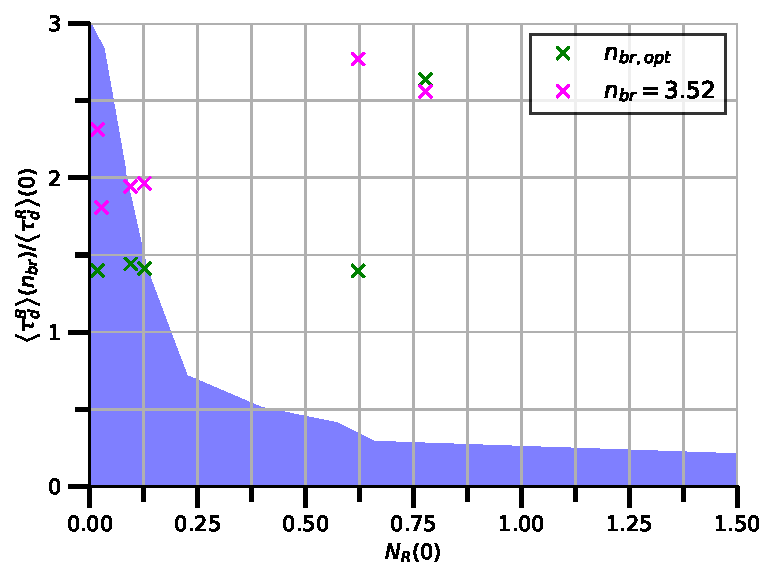
\includegraphics[width=4.8in]{ReferenceGraphValidation_Blue.pdf}
	\caption[Positions of validation measurements in application range illustration for blue channel]{Position of the validation experiments for the optimal brightness threshold (see Table~\ref{Table:ValidationOpt_Blue}) and for $n_{br} = \num{3.52}$ (see Table~\ref{Table:Validation_Blue}) in the illustration of the application range of the chance coincidence fraction for the blue channel. Only the first two measurements lie inside the application range. For the other measurement rows, the corrected coincidence fraction and its uncertainty increases systematically.}
	\label{fig:ReferenceGraphValidation_Blue}
\end{figure}
\vfill